\chapter{Developing an SMT Model (Moses)}
Moses is one of the most used SMT systems. It is a complete SMT system with a built-in decoder that can be used with several alignment algorithms. Moses is the SMT system that I used to train my English to Kinyarwanda translation model. In the next section, I describe the steps I followed to develop, train, and test my model using Moses. 
\section{Building a Baseline System}
After successfully installing Moses and other required software (Giza++, Boost, etc), I used it to train my English to Kinyarwanda translation model by using the \textit{King James Version}(KJV) Bible as my English corpus, and the \textit{Bibiliya Yera},  the Kinyarwanda translation of the KJV, as my Kinyarwanda corpus. 

%The following is a snippet of parallel verses extracted from the books of Psalms $119,\:1-2$. The English part is an extract from the \textit{King James Version} Bible and the Kinyarwanda part was extracted from the \textit{Bibiliya Yera}, the translation of the KJV.
%\begin{lstlisting}[breaklines]
    %Blessed are the undefiled in the way | Hahirwa abagenda batunganye
    %Who walk in the law of the Lord | Bakagendera mu mategeko y'Uwiteka
    %Blessed are they that keep his testimonies | Hahirwa abitondera ibyo yahamije
    %And that seek him with the whole heart | Bakamushakisha umutima wose
%\end{lstlisting}

The following is an excerpt of the first three verses of the New Testament in both the Kinyarwanda \textit{Bibiliya Yera} and the English \textit{King James Version} Bible (Matthew 1: 1-3). 
\begin{lstlisting}[breaklines]
1:1 Amasekuruza ya Yesu Kristo, mwene Dawidi, mwene Aburahamu ngaya: | 1:1 The book of the generation of Jesus Christ, the son of David, the son of Abraham.
1:2 Aburahamu yabyaye Isaka, Isaka yabyaye Yakobo, Yakobo yabyaye Yuda na bene se, | 1:2 Abraham begat Isaac; and Isaac begat Jacob; and Jacob begat Judas and his brethren;
1:3 Yuda yabyaye Peresi na Zera kuri Tamari, Peresi yabyaye Hesironi, Hesironi yabyaye Ramu, | 1:3 And Judas begat Phares and Zara of Thamar; and Phares begat Esrom; and Esrom begat Aram;
\end{lstlisting}

As you can see from the above excerpt of a parallel corpus, you need to have two files two equivalent texts in two languages: the target language and the source language. The content in those two files need to correspond line by line. Line 100 in the target language's file should be the translation of line 100 in the file containing the source language. In my case, as I was trying to build an English to Kinyarwanda translation system, I started with two different files, one containing the \textit{Bibiliya Yera} and the other one containing the \textit{King James Version} Bible. When using Moses, the first step in training a translation model is a process called \textit{``Corpus Preparation''}.
%%%%%%%
\subsection{Corpus Preparation}
Corpus Preparation consists of three steps: tokenization, truecasing, and cleaning.

During tokenization, spaces are added between all words and punctuation to make sure that different forms of the same word are counted as one. Without this step, the string ``God'', for example,  would be considered to be different from the string ``God!''. To avoid this kind of behavior that would result in \textit{data sparsity}, the \textit{Moses tokenizer} adds an extra space  in ``God!'' to make it ``God !''; thus, when frequencies of the word ``God'' are calculated, the Moses engine is able to return a correct count that contains all the occurrences of ``God!'', ``God,'', etc.

In the next step, Moses uses a \textit{truecasing} script, also known as the \textit{truecaser}, to calculate the frequencies ratios of how many times a certain word is lower-cased compared to when it is capitalized. This is important as without this step, it would be almost impossible for the translation system to guess if the words at the beginning of a sentence are capitalized because they are normally capitalized (proper names) or if they are capitalized just because they are the at the beginning of their respective sentences.

For example, the word ``God'' and ``god'' have two different meanings and those two meanings should be handled correctly by the translator. However, when ``God'' is used at the beginning of a sentence, the translator can't know for sure if it is capitalized because it is meant to be ``God'' or if it is the word ``god'' that is capitalized because it is at the beginning of a sentence. In this case, the \textit{Moses truecaser} trades off the $100\%$ uncertainty for a statistical guess based on the frequencies of both strings in the corpus. In an instance in which the frequency of the word ``God'' in the corpus is less than that of the string ``god'', all occurrences of ``God'' at the beginning of sentence will changed to ``god'', otherwise there will be no change. This is done for all words in the corpus and it helps to ensure that all meanings associated with capitalization are not all lost during the translation process. 

The last but very important step is the cleaning step. In this step, a sentence pair is removed from the training data if one of its sentences has a character count greater than a set amount, or if the ratio of the character counts of its sentences is not proportional to the calculated or set ratio for the training data. The limiting character count is set according to the structure of the languages that are being dealt with or the quality/size of the parallel corpora being used. 

In my case, I set to the character count to 180, which is very high compared to the ones used in the Moses tutorials that I looked at\cite{koehn2010moses, mosesbaselinesystem}. The reason why I set the limiting character count of my translation system to a larger number is because Bible verses tend to be very long than normal sentences used in conversations and discussions, two major sources of data used in the above-mentioned Moses tutorials.\cite{koehn2010moses, mosesbaselinesystem}.

In addition to that, I am confident that the verse-by-verse translations that I used to train my model are correct as they are from the Bible, and thus have been proofread by humans. In addition, as the main goal of this step is to remove incorrect translations, and I am more than confident in the literary accuracy of training data I used, setting a lower limiting character count for my translation model would not had improved my model at all, it would actually have caused more data scarcity, and that would reduce the overall accuracy of my model.

Below are the first three verses (Matthew 1: 1-3) from the \textit{King James Version} Bible after going through the three steps of the \textit{``Corpus Preparation''} process.
\begin{lstlisting}
1 : 1 The book of the generation of Jesus Christ , the son of David , the son of Abraham .
1 : 2 Abraham begat Isaac ; and Isaac begat Jacob ; and Jacob begat Judas and his brethren ;
1 : 3 And Judas begat Phares and Zara of Thamar ; and Phares begat Esrom ; and Esrom begat Aram ;
\end{lstlisting}

%%%%%%%%%%%%%%
\subsection{Language Model Training}
Target language model training is the following step after corpus preparation. In this step, I used Moses' built-in KenLM 3-gram model tool to construct a target language mode based on my corpus. In this case, as I am working with an English to Kinyarwanda translation, Kinyarwanda is my target language, thus I am going to use the \textit{Bibiliya Yera} corpus file generated the \textit{truecaser}. At this point, there is no need of using the output generated after the cleaning stage of the \textit{Corpus Preparation} process as a language model only depends on the structure of the target language being used, Kinyarwanda in this case, and not to its equivalent translation to the source language,  English in this case. Therefore there is no need to take into consideration the effects of the sentence character count and the limiting ratio used to filter data in the cleaning stage of the \textit{Corpus Preparation} process. After building the Kinyarwanda language model, I used the \textit{Moses binarizing script} to turn the file containing the Kinyarwanda language model into a binary version that loads faster. At this step, I can use it to get the probability that any input sentence is part of the Kinyarwanda according to the language model that I built using data solely from the \textit{Bibiliya Yera}. 
\begin{figure}[h]
\begin{center}
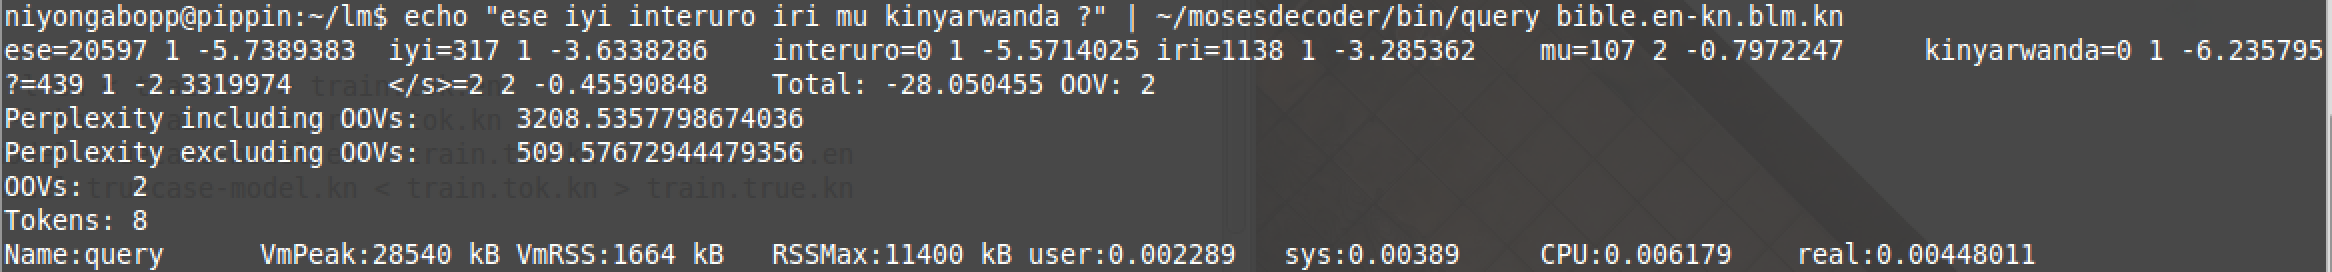
\includegraphics[width=4in]{figures/testing-a-lm}
\caption{Checking if the sentence ``ese iyi nteruro iri mu kinyarwanda ?'' (``is this sentence in kinyarwanda ?'') is indeed in Kinyarwanda according to a language model developed using corpus text from the \textit{Bibiliya Yera}.}
\end{center}
\end{figure}
\subsection{Training the Translation System}
Now that we have trained our target language model, it is time to start training the translation system. For this step, I used Moses default word-alignment tool called Giza++. After running the commands for this step, \textit{Moses} generated a \texttt{Moses.ini} configuration file that can be used to translate any English sentence to Kinyarwanda. However, at this point, there are two main issues that must be looked at. The first one is that translation takes a long time; to fix this we need to binarise the \textit{phrase and reordering tables}. The second one is that weights in our model configuration file are not adjusted, i.e.: they are dependent to the Bible data we used in training the model. In the next subsection, I talk about the process of tuning our model to make it more balanced and less dependent on the data used to train it.
%%%%%%%%%%%
\subsection{Tuning the Translation Model}
To tune our model, we need a separate small parallel corpus of high quality to add statistical variety to our model. The tuning process is important as it helps in making the translation model more balanced and less biased towards the data that was used during the training step. For example, as we only used data from the Bible, our model has only seen sentence structures, expressions, and words' combinations that are common in the Bible and nothing else from the commonly used conversational and/or formal language. Therefore, to make our model more efficient, it is crucial that we tune it using data that is very different from the Bible. As I couldn't easily find good-quality English data that is also translated in Kinyarwanda, I used the Rwandan constitution as it is freely-available on the web both in Kinyarwanda and in English. In the tuning process, as in the training process, I completed the steps of the \textit{corpus preparation} process on the tuning corpus data before using it. I ran the tuning process by using the minimum error rate training (MERT) algorithm\cite{och2003minimum}, the default option in \textit{Moses}\cite{mosesfactoredtraining}. I also performed this step in a newly created folder to avoid overwriting my previous model's configuration files.


\subsection{Binarising Phrase and Reordering Tables}
Once the tuning process is over, it is advised to binarise the \textit{phrase and reordering tables} in your translation model by using the Moses' built-in tools specialized for this process\cite{mosesbaselinesystem}.
\begin{figure}[h]
\begin{center}
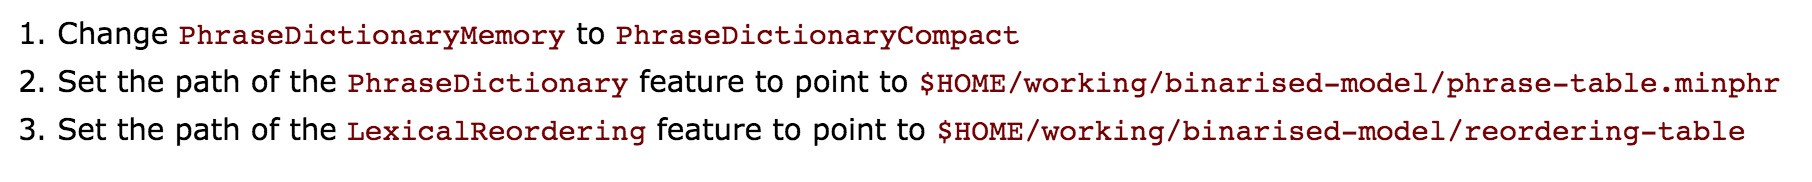
\includegraphics[width=4in]{figures/change-variables}
\caption{Examples of changes made to the \texttt{Moses.ini} configuration file to make sure it correctly points to the \textit{binarised} tables and the \textit{binarised} model directory.}
\end{center}
\end{figure}
\subsection{Testing the Translation Model}
Now that we have completed the basic steps of building, training, and tuning a translation model using \textit{Moses}, we can use it to do some simple translations. To do this, all you have to do is running terminal command, and that way you can translate a file containing sentences in English to Kinyarwanda. The sentences in the input file have to be in the same format as the ones in parallel corpora used in the training and tuning stages.

Below is the content of the English input file that I used to test my translation system followed by the Kinyarwanda file content that was generated the translator. \newline


\lstinputlisting[numbers=left]{files/input.txt}
\lstinputlisting[numbers=left]{files/output.txt}
\clearpage
\section{Translation Results}
As it can be seen from the results on the previous page, my translation system is still struggling with the translation of content that is not from the Bible. It can also be seen that it is almost incapable of translating long sentences as the one in line $5$. However, I am still hopeful that it can be improved by using more data. The data I used to train and tune  my translation model is like a drop in the ocean compared to the recommended quality and size as stressed by Och\cite{och2005statistical}.

It should also be noticed that even though the quality of my translation results if of low quality, the results I am getting are consistent with the parallel corpora I used to train and tune my translation model. As I used the Bible in the training process, one should expect my model to do well on translating sentences from the Bible. To a certain degree, that is what my model is doing but with an slightly lower accuracy rate. I suspect that is mainly caused by two reasons. 

The first one is that SMT systems work by using mathematical probabilities and decoding algorithms and not by directly looking up of each sentence in a large catalog of translations. The benefits of this is that SMTs systems are capable of translating sentences they have never seen before. However this comes at a cost that in some instances, the SMT model will return an incorrect translation for a sentence contained in the data that was used to train it.

\lstinputlisting[numbers=left, caption={Translation output of the English text on page $18$ when using a translation model both trained and tuned using content from the Bible.}]{files/example6.txt}
%\footnote{I used Psalms 119 because it is the longest chapter in the Bible and because it is made up of shorter sentences.}


The second reason why my translation isn't doing well as expected at translating sentences from the Bible is because I used data from the Rwandan Constitution in the tuning process. I did that hoping that tuning my translation model using external data would help improve the overall performance of the model, however it is hard to judge that with the results I have right now because my corpora sizes are too small to have a significant impact. The only thing that I am sure of is that tuning reduced the accuracy of my model for translations of sentences from the Bible. This is illustrated by the sentences in the example in Listing $3.1$ which are better translations of the input file than the results displayed on page $18$.


Another important thing to notice is that my translator, like other SMT-based translation systems, is incapable of inferring the difference of homonym words. For example, when I tried to translate ``It’s not that I’m so smart, it’s just that I stay with problems longer'', a quote attributed to Albert Einstein, my translator translated the word ``just'' as ``umukiranutsi'', the Kinyarwanda translation for ``a fair'' or  `` an impartial'' person! This shows that even though SMT-based translation systems perform better than rule-based systems, SMT is still inferior to human translation especially when it comes to these kind of situations in which words with the same spelling have more than one meaning.
\clearpage
